\documentclass[a4paper,oneside,DIV=12,12pt,headings=normal]{scrartcl}

%%% Length calculations
\usepackage{calc}
%%%

%%% Support for color
\usepackage{xcolor}
\definecolor{lightblue}{HTML}{03A9F4}
\definecolor{red}{HTML}{F44336}
%%%

%%% Graphics inclusion
\usepackage{graphicx}
%%%

%%% Font selection
\usepackage{fontspec}

\setromanfont{STIX Two Text}[
	SmallCapsFeatures = {LetterSpace = 5},
]

\setsansfont{Source Sans Pro}[
]

\setmonofont{Source Code Pro}[
]
%%%

%%% Math settings
\usepackage{amsmath,unicode-math}
\setmathfont{STIX Two Math}

\usepackage{IEEEtrantools}
\usepackage{mleftright}
%%%

%%% Font settings for different KOMA Script elements
\setkomafont{pagenumber}{\rmfamily}
\setkomafont{disposition}{\rmfamily\bfseries}
%%%

%%% Typographic enhancements
\usepackage{microtype}
%%%

%%% Language-specific settings
\usepackage{polyglossia}
\setmainlanguage{ukrainian}
%%%

%%% List settings
\usepackage{enumitem}
\setlist[enumerate]{
	leftmargin = *,
}
%%%

%%% Captions
\usepackage{caption}
\usepackage{subcaption}

\DeclareCaptionLabelFormat{closing}{#2)}
\captionsetup[subtable]{labelformat = closing}
\captionsetup[subfigure]{labelformat = closing, position = auto}
%%%

%%% Tables
\usepackage{booktabs}
\usepackage{longtable}

\usepackage{multirow}

\usepackage{array}
\newcolumntype{v}[1]{>{\raggedright\arraybackslash\hspace{0pt}}p{#1}}
\newcolumntype{b}[1]{>{\centering\arraybackslash\hspace{0pt}}p{#1}}
\newcolumntype{n}[1]{>{\raggedleft\arraybackslash\hspace{0pt}}p{#1}}

\usepackage{kbordermatrix} % labeling array indices
%%%

%%% Floats on a single row
% \usepackage{floatrow}
% \newfloatcommand{capbtabbox}{table}[][\FBwidth]
%%%

%%% Links and hyperreferences
\usepackage{hyperref}
\hypersetup{
	colorlinks      = false,
	linkbordercolor = red,
	urlbordercolor  = lightblue,
	pdfborderstyle  = {/S/U/W 1.5},
}
%%%

%%% All caps
\newcommand{\allcaps}[1]{{\addfontfeatures{LetterSpace = 3}#1}}
%%%

\setlength{\emergencystretch}{1em}

\begin{document}
	\begin{titlepage}
	\centering
		Міністерство освіти і~науки України\\
		Національний авіаційний університет\\
		Навчально-науковий інститут комп'ютерних інформаційних технологій\\
		Кафедра комп'ютеризованих систем управління

		\vspace*{\fill}

		Лабораторна робота №5\\
		з дисципліни «Комп'ютерна схемотехніка»\\
		на тему «Дослідження кодоперетворювачів»

		\vspace*{\fill}
		
		\begin{flushright}
			Виконав:\\
			студент ННІКІТ СП-225\\
			Клокун В.\,Д.\\
			Перевірив:\\
			Іскренко Ю.\,Ю.
		\end{flushright}

		Київ 2018
	\end{titlepage}

	\section{Мета роботи}
		Вивчення логіки роботи, принципів побудови й синтезу схем перетворювачів кодів. Визначення основних характеристик перетворювачів кодів на~інтегральних мікросхемах. Ознайомлення з мікросхемами перетворювачів кодів у серіях інтегральних мікросхем.

	\section{Хід роботи}
		\subsection{Дослідження схеми 4-розрядного перетворювача прямого~коду у~зворотній~код}
			Записуємо систему рівнянь у вигляді, зручному для реалізації на елементах І—АБО—НІ на основі виразу $Y_{\text{ЗН}} = X_{\text{ЗН}}$:
			\begin{IEEEeqnarray*}{l}
				Y_3 = \neg \left( X_{\text{ЗН}} \land X_3 \lor \neg X_{\text{ЗН}} \land \neg X_3 \right), \\
				Y_2 = \neg \left( X_{\text{ЗН}} \land X_2 \lor \neg X_{\text{ЗН}} \land \neg X_2 \right), \\
				Y_1 = \neg \left( X_{\text{ЗН}} \land X_1 \lor \neg X_{\text{ЗН}} \land \neg X_1 \right).
			\end{IEEEeqnarray*}

			Збираємо схему 4-розрядного (з урахуванням знаку) перетворювача прямого коду у зворотній~(рис.~\ref{fig:01-4digit-str-to-1s-complement}), згідно з системою рівнянь на логічних елементах І—АБО—НІ та НЕ—І. Подаємо на входи перетворювача значення вхідного коду і записуємо результат перетворення~(табл.~\ref{tab:01-transformation}).
			\begin{figure}[!htbp]
				\centering
				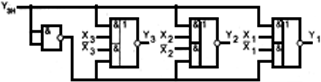
\includegraphics[width = 0.66\linewidth]{./assets/01.png}
				\caption{Схема 4-розрядного перетворювача прямого коду у зворотній}
				\label{fig:01-4digit-str-to-1s-complement}
			\end{figure}


		\subsection{Дослідження схеми 4-розрядного перетворювача прямого~коду у~додатковий~код}
			Записуємо систему рівнянь у вигляді, зручному для реалізації на елементах І—АБО—НІ на основі виразу $Y_{\text{ЗН}} = X_{\text{ЗН}}$:
			\begin{IEEEeqnarray*}{rCl}
				Y_3 &=& X_3 \oplus \left( X_2 \lor X_1 \right)\\
						&=& \neg \left( \neg X_3 \land
						  \neg \left(
								X_2 \land X_{\text{ЗН}} \lor X_1 \land X_{\text{ЗН}}
							\right)
							\lor
							X_3 \land
							\left(
								X_2 \land X_{\text{ЗН}} \lor X_1 \land X_{\text{ЗН}}
							\right)
						\right),\\
				Y_2 &=& \neg \left(
				      \neg X_3 \land
							\neg \left(
							X_2 \land X_{\text{ЗН}}
							\right)
							\lor
							X_3 
							\land
							\left(
							X_2 \land X_{\text{ЗН}}
							\lor
							X_1 \land X_{\text{ЗН}}
							\right)
				      \right),\\
					Y_1 &=& X_1.
			\end{IEEEeqnarray*}

			Збираємо схему 4-розрядного (з урахуванням знаку) перетворювача прямого коду у додатковий~(рис.~\ref{fig:01-4digit-str-to-2s-complement}), згідно з системою рівнянь на логічних елементах І—АБО—НІ та НЕ—І. Подаємо на входи перетворювача значення вхідного коду і записуємо результат перетворення~(табл.~\ref{tab:01-transformation}).
			\begin{figure}[!htbp]
				\centering
				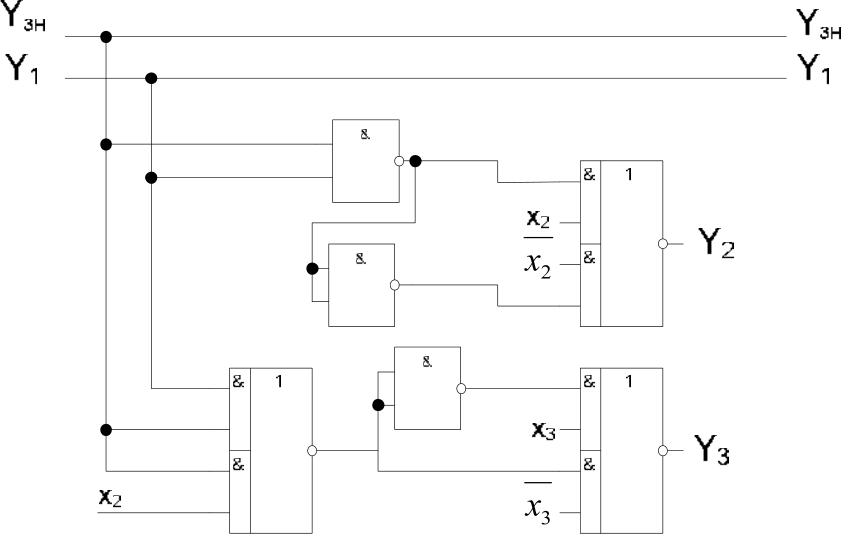
\includegraphics[width = 0.66\linewidth]{./assets/02.png}
				\caption{Схема 4-розрядного перетворювача прямого коду у додатковий}
				\label{fig:01-4digit-str-to-2s-complement}
			\end{figure}

			\begin{table}[!htbp]
				\centering
				\begin{tabular}{llrllr}
					\toprule
						$Y_{\text{пр}}$ & $Y_{\text{об}}$ & $Y_{\text{доп}}$ & $Y_{\text{пр}}$ & $Y_{\text{об}}$ & $Y_{\text{доп}}$ \\
					\midrule
						0.000 & & & 1.000 & & \\
						0.001 & & & 1.001 & & \\
						0.010 & & & 1.010 & & \\
						0.011 & & & 1.011 & & \\
						0.100 & & & 1.100 & & \\
						0.101 & & & 1.101 & & \\
						0.110 & & & 1.110 & & \\
						0.111 & & & 1.111 & & \\
					\bottomrule
				\end{tabular}
				\caption{Результати перетворень}
				\label{tab:01-transformation}
			\end{table}

		\subsection{Дослідження схеми 4-розрядного перетворювача двійкового~числа у~код~Грея}
			Записуємо систему рівнянь у вигляді, зручному для реалізації на елементах І—АБО—НІ:
			\begin{IEEEeqnarray*}{rCl}
				I_1 &=& X_1 \oplus X_2
				        = \neg \left( \neg X_1 \land \neg X_2 \lor X_2 \land X_1\right),\\
				I_2 &=& X_2 \oplus X_3
				        = \neg \left( \neg X_2 \land \neg X_3 \lor X_2 \land X_3 \right),\\
				I_3 &=& X_3 \oplus X_4
				        = \neg \left( \neg X_3 \land \neg X_4 \lor X_3 \land X_4 \right),\\
				I_4 &=& X_4.
			\end{IEEEeqnarray*}

			Збираємо схему 4-розрядного перетворювача двійкового числа в код Грея на логічних елементах І—АБО—НІ~(рис.~\ref{fig:03-binary-to-gray-code}). Подаємо на входи перетворювача значення вхідного коду і порівнюємо результати перетворення з теоретичними даними~(табл.~\ref{tab:03-binary-to-gray-code}).
			\begin{figure}[!htbp]
				\centering
				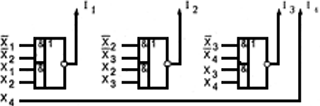
\includegraphics[width = 0.66\linewidth]{./assets/03.png}
				\caption{Схема перетворювача двійкового числа в код Грея}
				\label{fig:03-binary-to-gray-code}
			\end{figure}
			
			\begin{table}[!htbp]
				\centering
				\begin{tabular}{*{4}{l}*{4}{r}}
					\toprule
						$X_4$ & $X_3$ & $X_2$ & $X_1$ & $I_4$ & $I_3$ & $I_2$ & $I_1$ \\
					\midrule
					  0     & 0     & 0     & 0     & 0     & 0     & 0     & 0     \\
					  0     & 0     & 0     & 1     & 0     & 0     & 0     & 1     \\
					  0     & 0     & 1     & 0     & 0     & 0     & 1     & 1     \\
					  0     & 0     & 1     & 1     & 0     & 0     & 1     & 0     \\
					  0     & 1     & 0     & 0     & 0     & 1     & 1     & 0     \\
					  0     & 1     & 0     & 1     & 0     & 1     & 1     & 1     \\
					  0     & 1     & 1     & 0     & 0     & 1     & 0     & 1     \\
					  0     & 1     & 1     & 1     & 0     & 1     & 0     & 0     \\
					  1     & 0     & 0     & 0     & 1     & 1     & 0     & 0     \\
					  1     & 0     & 0     & 1     & 1     & 1     & 0     & 1     \\
					  1     & 0     & 1     & 0     & 1     & 1     & 1     & 1     \\
					  1     & 0     & 1     & 1     & 1     & 1     & 1     & 0     \\
					  1     & 1     & 0     & 0     & 1     & 0     & 1     & 0     \\
					  1     & 1     & 0     & 1     & 1     & 0     & 1     & 1     \\
					  1     & 1     & 1     & 0     & 1     & 0     & 0     & 1     \\
					  1     & 1     & 1     & 1     & 1     & 0     & 0     & 0     \\
					\bottomrule
				\end{tabular}
				\caption{Результат перетворень двійкових чисел в код Грея}
				\label{tab:03-binary-to-gray-code}
			\end{table}

		\subsection{Дослідження схеми 4-розрядного формувача~кодів}
			Записуємо систему рівнянь для мікрооперації $Y_1$—$Y_4$ у вигляді, зручному для реалізації на логічних елементах НЕ—І за умови, що $Z_1 = Y_1 \lor Y_2$ і~$Z_2 = Y_3 \lor Y_4$:
			{\allowdisplaybreaks
			\begin{IEEEeqnarray*}{rCl}
				F_1 &=& \neg \left( \neg \left( Z_1 \lor Z_2 \land X_1 \right) \right)
				        = \neg \left( \neg Z_1 \land \neg \left( Z_2 \land X_1 \right) \right),\\
				F_2 &=& \neg \left( \neg \left( Z_1 \lor Z_2 \land X_2 \right) \right)
				        = \neg \left( \neg Z_1 \land \neg \left( Z_2 \land X_2 \right) \right),\\
				F_3 &=& \neg \left( \neg \left( Z_1 \lor Z_2 \land X_3 \right) \right)
				        = \neg \left( \neg Z_1 \land \neg \left( Z_2 \land X_3 \right) \right),\\
				F_4 &=& \neg \left( \neg \left( Y_1 \lor Y_3 \land X_4 \right) \right)
				        = \neg \left( \neg Y_1 \land \neg \left( Y_3 \land X_4 \right) \right).
			\end{IEEEeqnarray*}}

			Збираємо схему формувача кодів на елементах НЕ—І~(рис.~\ref{fig:04-codegen}). Подаємо на входи формувача кодів значення двійкового числа~$A$ для керуючих сигналів~$Y_1$—$Y_4$~(сигналів мікрооперацій, табл.~\ref{tab:04-transformation}) і записуємо вихідний код.
			\begin{figure}[!htbp]
				\centering
				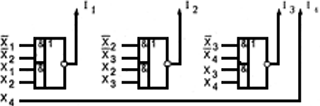
\includegraphics[width = 0.66\linewidth]{./assets/03.png}
				\caption{Схема формувача кодів}
				\label{fig:04-codegen}
			\end{figure}

			\begin{table}[!htbp]
				\centering
				\begin{tabular}{ll*{4}{r}}
					\toprule
						$Y_i$ & $A$   & $F_4$ & $F_3$ & $F_2$ & $F_1$ \\
					\midrule
						$Y_1$ & 0.010 &       &       &       & \\
						$Y_1$ & 1.101 &       &       &       & \\
						$Y_2$ & 1.111 &       &       &       & \\
						$Y_2$ & 0.000 &       &       &       & \\
						$Y_3$ & 0.010 &       &       &       & \\
						$Y_3$ & 1.100 &       &       &       & \\
						$Y_4$ & 1.101 &       &       &       & \\
						$Y_4$ & 1.011 &       &       &       & \\
					\bottomrule
				\end{tabular}
				\caption{Результати формування кодів}
				\label{tab:04-transformation}
			\end{table}

		\subsection{Дослідження схеми перетворювача Д-кода у~зворотній~код}
			Д-код~(зважений Д-код, двійково-десятковий код, binary-coded decimal, \allcaps{BCD})~— це код, в якому кожна десяткова цифра (0, 1,~…, 9) замінюється її чотирибітним двійковим еквівалентом~(0000, 0001,~…, 1001). Наприклад: $729_{10} = 0111 0010 1001_{2-10}$. Особливістю Д-кодів є наявність 10~дозволених і~6~заборонених комбінацій. Поява забороненої комбінації при виконанні операцій над числами свідчить про виникнення помилки або ж про необхідність корекції результату.

			Записуємо співвідношення у вигляді, зручному для реалізації на логічних елементах І—АБО—НІ та НЕ—І:
			\begin{IEEEeqnarray*}{l}
				Y_1 = \neg X_1,\quad  Y_2 = X_2,\quad
				Y_3 = \neg \left( \neg X_2 \land \neg X_3 \lor X_2 \land X_3 \right),\quad Y_4 = \neg X_4 \land \neg X_3 \land \neg X_3.
			\end{IEEEeqnarray*}

			Збираємо схему перетворювача Д-кода у зворотній код на елементах І—АБО—НІ та НЕ—І~(рис.~\ref{fig:05-d-code}). Подаємо на входи перетворювача значення Д-кода і записуємо результати перетворення~(табл.~\ref{tab:05-d-code-transformation}).
			\begin{figure}[!htbp]
				\centering
				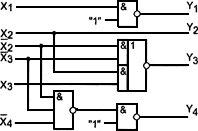
\includegraphics[width = 0.33\linewidth]{./assets/05.png}
				\caption{Схема перетворювача Д-кода у зворотній код}
				\label{fig:05-d-code}
			\end{figure}

			\begin{table}[!htbp]
				\centering
				\begin{tabular}{l*{4}{r}}
					\toprule
						$X$  & $Y_4$ & $Y_3$ & $Y_2$ & $Y_1$ \\
					\midrule
						0000 &       &       &       & \\
						0001 &       &       &       & \\
						0010 &       &       &       & \\
						0011 &       &       &       & \\
						0100 &       &       &       & \\
						0101 &       &       &       & \\
						0110 &       &       &       & \\
						0111 &       &       &       & \\
						1000 &       &       &       & \\
						1001 &       &       &       & \\
					\bottomrule
				\end{tabular}
				\caption{Результати перетворення Д-кода у зворотній код}
				\label{tab:05-d-code-transformation}
			\end{table}


	\section{Висновок}
		Виконуючи дану лабораторну роботу, ми вивчили логіку роботи, принципи побудови й синтезу схем перетворювачів кодів; визначили основні характеристики перетворювачів кодів на~інтегральних мікросхемах; ознайомились з мікросхемами перетворювачів кодів у серіях інтегральних мікросхем.

\end{document}

